\documentclass[14pt]{extarticle}

\usepackage[T1,T2A]{fontenc}
\usepackage[utf8]{inputenc}
\usepackage[english,ukrainian]{babel}
\usepackage{graphicx}
\usepackage{framed}
\usepackage[normalem]{ulem}
\usepackage{indentfirst}
\usepackage{amsmath,amsthm,amssymb,amsfonts}
\usepackage{float}
\usepackage[italicdiff]{physics}
%\usepackage{pifont} %For unusual symbols
%\usepackage{mathdots} %For unusual combinations of dots
\usepackage{wrapfig}
\usepackage[inline,shortlabels]{enumitem}

\usepackage[dvipsnames]{xcolor}
\usepackage[utf8]{inputenc}
\usepackage[a4paper, top=1in,bottom=1in, left=1in, right=1in, footskip=0.3in, includefoot]{geometry}
\usepackage[most]{tcolorbox}
\usepackage{tikz,tikz-3dplot,tikz-cd,tkz-tab,tkz-euclide,pgf,pgfplots}
\pgfplotsset{compat=newest}
\usepackage{multicol}
\usepackage[bottom,multiple]{footmisc} %ensures footnotes are at the bottom of the page, and separates footnotes by a comma if they are adjacent
\usepackage{hyperref}
\usepackage[nameinlink]{cleveref} %nameinlink ensures that the entire element is clickable in the pdf, not just the number

\newcommand{\remind}[1]{\textcolor{red}{\textbf{#1}}} %To remind me of unfinished work to fix later
\newcommand{\hide}[1]{} %To hide large blocks of code without using % symbols

\newcommand{\ep}{\varepsilon}
\newcommand{\vp}{\varphi}
\newcommand{\lam}{\lambda}
\newcommand{\Lam}{\Lambda}
%\newcommand{\abs}[1]{\ensuremath{\left\lvert#1\right\rvert}} % This clashes with the physics package
%\newcommand{\norm}[1]{\ensuremath{\left\lVert#1\right\rVert}} % This clashes with the physics package
\renewcommand{\ip}[1]{\ensuremath{\left\langle#1\right\rangle}}
\newcommand{\floor}[1]{\ensuremath{\left\lfloor#1\right\rfloor}}
\newcommand{\ceil}[1]{\ensuremath{\left\lceil#1\right\rceil}}
\newcommand{\A}{\mathbb{A}}
\newcommand{\B}{\mathbb{B}}
\newcommand{\D}{\mathbb{D}}
\newcommand{\E}{\mathbb{E}}
\newcommand{\F}{\mathbb{F}}
\newcommand{\K}{\mathbb{K}}
\newcommand{\N}{\mathbb{N}}
\newcommand{\Q}{\mathbb{Q}}
\newcommand{\R}{\mathbb{R}}
\newcommand{\T}{\mathbb{T}}
\newcommand{\X}{\mathbb{X}}
\newcommand{\Y}{\mathbb{Y}}
\newcommand{\Z}{\mathbb{Z}}
\newcommand{\As}{\mathcal{A}}
\newcommand{\Bs}{\mathcal{B}}
\newcommand{\Cs}{\mathcal{C}}
\newcommand{\Ds}{\mathcal{D}}
\newcommand{\Es}{\mathcal{E}}
\newcommand{\Fs}{\mathcal{F}}
\newcommand{\Gs}{\mathcal{G}}
\newcommand{\Hs}{\mathcal{H}}
\newcommand{\Is}{\mathcal{I}}
\newcommand{\Js}{\mathcal{J}}
\newcommand{\Ks}{\mathcal{K}}
\newcommand{\Ls}{\mathcal{L}}
\newcommand{\Ms}{\mathcal{M}}
\newcommand{\Ns}{\mathcal{N}}
\newcommand{\Os}{\mathcal{O}}
\newcommand{\Ps}{\mathcal{P}}
\newcommand{\Qs}{\mathcal{Q}}
\newcommand{\Rs}{\mathcal{R}}
\newcommand{\Ss}{\mathcal{S}}
\newcommand{\Ts}{\mathcal{T}}
\newcommand{\Us}{\mathcal{U}}
\newcommand{\Vs}{\mathcal{V}}
\newcommand{\Ws}{\mathcal{W}}
\newcommand{\Xs}{\mathcal{X}}
\newcommand{\Ys}{\mathcal{Y}}
\newcommand{\Zs}{\mathcal{Z}}
\newcommand{\ab}{\textbf{a}}
\newcommand{\bb}{\textbf{b}}
\newcommand{\cb}{\textbf{c}}
\newcommand{\db}{\textbf{d}}
\newcommand{\ub}{\textbf{u}}
%\renewcommand{\vb}{\textbf{v}} % This clashes with the physics package (the physics package already defines the \vb command)
\newcommand{\wb}{\textbf{w}}
\newcommand{\xb}{\textbf{x}}
\newcommand{\yb}{\textbf{y}}
\newcommand{\zb}{\textbf{z}}
\newcommand{\Ab}{\textbf{A}}
\newcommand{\Bb}{\textbf{B}}
\newcommand{\Cb}{\textbf{C}}
\newcommand{\Db}{\textbf{D}}
\newcommand{\eb}{\textbf{e}}
\newcommand{\ex}{\textbf{e}_x}
\newcommand{\ey}{\textbf{e}_y}
\newcommand{\ez}{\textbf{e}_z}
\newcommand{\abar}{\overline{a}}
\newcommand{\bbar}{\overline{b}}
\newcommand{\cbar}{\overline{c}}
\newcommand{\dbar}{\overline{d}}
\newcommand{\ubar}{\overline{u}}
\newcommand{\vbar}{\overline{v}}
\newcommand{\wbar}{\overline{w}}
\newcommand{\xbar}{\overline{x}}
\newcommand{\ybar}{\overline{y}}
\newcommand{\zbar}{\overline{z}}
\newcommand{\Abar}{\overline{A}}
\newcommand{\Bbar}{\overline{B}}
\newcommand{\Cbar}{\overline{C}}
\newcommand{\Dbar}{\overline{D}}
\newcommand{\Ubar}{\overline{U}}
\newcommand{\Vbar}{\overline{V}}
\newcommand{\Wbar}{\overline{W}}
\newcommand{\Xbar}{\overline{X}}
\newcommand{\Ybar}{\overline{Y}}
\newcommand{\Zbar}{\overline{Z}}
\newcommand{\Aint}{A^\circ}
\newcommand{\Bint}{B^\circ}
\newcommand{\limk}{\lim_{k\to\infty}}
\newcommand{\limm}{\lim_{m\to\infty}}
\newcommand{\limn}{\lim_{n\to\infty}}
\newcommand{\limx}[1][a]{\lim_{x\to#1}}
\newcommand{\liminfm}{\liminf_{m\to\infty}}
\newcommand{\limsupm}{\limsup_{m\to\infty}}
\newcommand{\liminfn}{\liminf_{n\to\infty}}
\newcommand{\limsupn}{\limsup_{n\to\infty}}
\newcommand{\sumkn}{\sum_{k=1}^n}
\newcommand{\sumk}[1][1]{\sum_{k=#1}^\infty}
\newcommand{\summ}[1][1]{\sum_{m=#1}^\infty}
\newcommand{\sumn}[1][1]{\sum_{n=#1}^\infty}
\newcommand{\emp}{\varnothing}
\newcommand{\exc}{\backslash}
\newcommand{\sub}{\subseteq}
\newcommand{\sups}{\supseteq}
\newcommand{\capp}{\bigcap}
\newcommand{\cupp}{\bigcup}
\newcommand{\kupp}{\bigsqcup}
\newcommand{\cappkn}{\bigcap_{k=1}^n}
\newcommand{\cuppkn}{\bigcup_{k=1}^n}
\newcommand{\kuppkn}{\bigsqcup_{k=1}^n}
\newcommand{\cappk}[1][1]{\bigcap_{k=#1}^\infty}
\newcommand{\cuppk}[1][1]{\bigcup_{k=#1}^\infty}
\newcommand{\cappm}[1][1]{\bigcap_{m=#1}^\infty}
\newcommand{\cuppm}[1][1]{\bigcup_{m=#1}^\infty}
\newcommand{\cappn}[1][1]{\bigcap_{n=#1}^\infty}
\newcommand{\cuppn}[1][1]{\bigcup_{n=#1}^\infty}
\newcommand{\kuppk}[1][1]{\bigsqcup_{k=#1}^\infty}
\newcommand{\kuppm}[1][1]{\bigsqcup_{m=#1}^\infty}
\newcommand{\kuppn}[1][1]{\bigsqcup_{n=#1}^\infty}
\newcommand{\cappa}{\bigcap_{\alpha\in I}}
\newcommand{\cuppa}{\bigcup_{\alpha\in I}}
\newcommand{\kuppa}{\bigsqcup_{\alpha\in I}}
\newcommand{\Rx}{\overline{\mathbb{R}}}
\newcommand{\dx}{\,dx}
\newcommand{\dy}{\,dy}
\newcommand{\dt}{\,dt}
\newcommand{\dax}{\,d\alpha(x)}
\newcommand{\dbx}{\,d\beta(x)}
\DeclareMathOperator{\glb}{\text{glb}}
\DeclareMathOperator{\lub}{\text{lub}}
\newcommand{\xh}{\widehat{x}}
\newcommand{\yh}{\widehat{y}}
\newcommand{\zh}{\widehat{z}}
\newcommand{\<}{\langle}
\renewcommand{\>}{\rangle}
\renewcommand{\iff}{\Leftrightarrow}
\DeclareMathOperator{\im}{\text{im}}
\let\spn\relax\let\Re\relax\let\Im\relax
\DeclareMathOperator{\spn}{\text{span}}
\DeclareMathOperator{\Re}{\text{Re}}
\DeclareMathOperator{\Im}{\text{Im}}
\DeclareMathOperator{\diag}{\text{diag}}

\newtheoremstyle{mystyle}{}{}{}{}{\sffamily\bfseries}{.}{ }{}
\newtheoremstyle{cstyle}{}{}{}{}{\sffamily\bfseries}{.}{ }{\thmnote{#3}}
\makeatletter
\renewenvironment{proof}[1][\proofname] {\par\pushQED{\qed}{\normalfont\sffamily\bfseries\topsep6\p@\@plus6\p@\relax #1\@addpunct{.} }}{\popQED\endtrivlist\@endpefalse}
\makeatother
\newcommand{\coolqed}[1]{\includegraphics[width=#1cm]{sunglasses_emoji.png}} %Defines the new QED symbol
\renewcommand{\qedsymbol}{\coolqed{0.32}} %Implements the new QED symbol
\theoremstyle{mystyle}{\newtheorem{definition}{Definition}[section]}
\theoremstyle{mystyle}{\newtheorem{proposition}[definition]{Proposition}}
\theoremstyle{mystyle}{\newtheorem{theorem}[definition]{Theorem}}
\theoremstyle{mystyle}{\newtheorem{lemma}[definition]{Lemma}}
\theoremstyle{mystyle}{\newtheorem{corollary}[definition]{Corollary}}
\theoremstyle{mystyle}{\newtheorem*{remark}{Remark}}
\theoremstyle{mystyle}{\newtheorem*{remarks}{Remarks}}
\theoremstyle{mystyle}{\newtheorem*{example}{Example}}
\theoremstyle{mystyle}{\newtheorem*{examples}{Examples}}
\theoremstyle{definition}{\newtheorem*{exercise}{Exercise}}
\theoremstyle{cstyle}{\newtheorem*{cthm}{}}

%Warning environment
\newtheoremstyle{warn}{}{}{}{}{\normalfont}{}{ }{}
\theoremstyle{warn}
\newtheorem*{warning}{\warningsign{0.2}\relax}

%Symbol for the warning environment, designed to be easily scalable
\newcommand{\warningsign}[1]{\tikz[scale=#1,every node/.style={transform shape}]{\draw[-,line width={#1*0.8mm},red,fill=yellow,rounded corners={#1*2.5mm}] (0,0)--(1,{-sqrt(3)})--(-1,{-sqrt(3)})--cycle;
\node at (0,-1) {\fontsize{48}{60}\selectfont\bfseries!};}}

\tcolorboxenvironment{definition}{boxrule=0pt,boxsep=0pt,colback={red!10},left=8pt,right=8pt,enhanced jigsaw, borderline west={2pt}{0pt}{red},sharp corners,before skip=10pt,after skip=10pt,breakable}
\tcolorboxenvironment{proposition}{boxrule=0pt,boxsep=0pt,colback={Orange!10},left=8pt,right=8pt,enhanced jigsaw, borderline west={2pt}{0pt}{Orange},sharp corners,before skip=10pt,after skip=10pt,breakable}
\tcolorboxenvironment{theorem}{boxrule=0pt,boxsep=0pt,colback={blue!10},left=8pt,right=8pt,enhanced jigsaw, borderline west={2pt}{0pt}{blue},sharp corners,before skip=10pt,after skip=10pt,breakable}
\tcolorboxenvironment{lemma}{boxrule=0pt,boxsep=0pt,colback={Cyan!10},left=8pt,right=8pt,enhanced jigsaw, borderline west={2pt}{0pt}{Cyan},sharp corners,before skip=10pt,after skip=10pt,breakable}
\tcolorboxenvironment{corollary}{boxrule=0pt,boxsep=0pt,colback={violet!10},left=8pt,right=8pt,enhanced jigsaw, borderline west={2pt}{0pt}{violet},sharp corners,before skip=10pt,after skip=10pt,breakable}
\tcolorboxenvironment{proof}{boxrule=0pt,boxsep=0pt,blanker,borderline west={2pt}{0pt}{CadetBlue!80!white},left=8pt,right=8pt,sharp corners,before skip=10pt,after skip=10pt,breakable}
\tcolorboxenvironment{remark}{boxrule=0pt,boxsep=0pt,blanker,borderline west={2pt}{0pt}{Green},left=8pt,right=8pt,before skip=10pt,after skip=10pt,breakable}
\tcolorboxenvironment{remarks}{boxrule=0pt,boxsep=0pt,blanker,borderline west={2pt}{0pt}{Green},left=8pt,right=8pt,before skip=10pt,after skip=10pt,breakable}
\tcolorboxenvironment{example}{boxrule=0pt,boxsep=0pt,blanker,borderline west={2pt}{0pt}{Black},left=8pt,right=8pt,sharp corners,before skip=10pt,after skip=10pt,breakable}
\tcolorboxenvironment{examples}{boxrule=0pt,boxsep=0pt,blanker,borderline west={2pt}{0pt}{Black},left=8pt,right=8pt,sharp corners,before skip=10pt,after skip=10pt,breakable}
\tcolorboxenvironment{cthm}{boxrule=0pt,boxsep=0pt,colback={gray!10},left=8pt,right=8pt,enhanced jigsaw, borderline west={2pt}{0pt}{gray},sharp corners,before skip=10pt,after skip=10pt,breakable}

%align and align* environments with inline size
\newenvironment{talign}{\let\displaystyle\textstyle\align}{\endalign}
\newenvironment{talign*}{\let\displaystyle\textstyle\csname align*\endcsname}{\endalign}

\usepackage[explicit]{titlesec}
\titleformat{\section}{\fontsize{24}{30}\sffamily\bfseries}{\thesection}{20pt}{#1}
\titleformat{\subsection}{\fontsize{16}{18}\sffamily\bfseries}{\thesubsection}{12pt}{#1}
\titleformat{\subsubsection}{\fontsize{10}{12}\sffamily\large\bfseries}{\thesubsubsection}{8pt}{#1}

\titlespacing*{\section}{0pt}{5pt}{5pt}
\titlespacing*{\subsection}{0pt}{5pt}{5pt}
\titlespacing*{\subsubsection}{0pt}{5pt}{5pt}

%\newcommand{\sectionbreak}{\clearpage} %Start every section on a new page

\newcommand{\Disp}{\displaystyle}
\newcommand{\qe}{\hfill\(\bigtriangledown\)}
\DeclareMathAlphabet\mathbfcal{OMS}{cmsy}{b}{n}
\setlength{\parindent}{0.2in}
\setlength{\parskip}{0pt}
\setlength{\columnseprule}{0pt}

\title{\huge\sffamily\bfseries Іспит з Комплексного Аналізу}
\author{\Large\sffamily Дмитра Захарова Олеговича. МП-31}
\date{\sffamily 3 червня 2024 р.}

\begin{document}

\maketitle

%Custom colors for different environments
\definecolor{contcol1}{HTML}{72E094}
\definecolor{contcol2}{HTML}{24E2D6}
\definecolor{convcol1}{HTML}{C0392B}
\definecolor{convcol2}{HTML}{8E44AD}

\begin{center}
    \textbf{Білет \#14}
\end{center}

\begin{tcolorbox}[title=Вміст, fonttitle=\sffamily\bfseries\selectfont,interior style={left color=contcol1!40!white,right color=contcol2!40!white},frame style={left color=contcol1!80!white,right color=contcol2!80!white},coltitle=black,top=2mm,bottom=2mm,left=2mm,right=2mm,drop fuzzy shadow,enhanced,breakable]
\makeatletter
\@starttoc{toc}
\makeatother
\end{tcolorbox}

\newpage

\textbf{Передумова.} Тут і далі будемо позначати через $\mathcal{H}(\mathcal{D})$  множину голоморфних функцій, а через $\mathcal{C}(\mathcal{D})$ -- клас неперервних функцій на заданій області $\mathcal{D} \subset \mathbb{C}$. Також, позначаємо $B_r(z_0) = \{z \in \mathbb{C}: |z-z_0|<r\}$.

\section{Теорема Морери}

\textbf{Відповідь.} Теорема Морери за своєю суттю є зворотньою до теореми Коші, тобто вона відповідає на питання: що саме потрібно від функції окрім неперервності, щоб вона була голоморфною. Сформуюємо її.

\begin{theorem}
\textbf{Теорема Морери.} Нехай $f(z) \in \mathcal{C}(\mathcal{D})$, а також для будь-якого замкненого контуру $\Gamma \subset \mathcal{D}$ виконується умова
\begin{equation}
    \oint_{\Gamma} f(z)dz = 0.
\end{equation}

Тоді, $f(z) \in \mathcal{H}(\mathcal{D})$.
\end{theorem}

\textbf{Доведення.} По-перше, доведемо наступну допоміжну лему.

\begin{lemma}
    Значення інтегралу $\int_a^b f(z)dz$ для $a,b \in \mathbb{C}$ не залежить від обраного шляху від $a$ до $b$.
\end{lemma}

\textbf{Доведення леми.} Дійсно, нехай є два шляхи $\ell_1,\ell_2$ від $a$ до $b$. В такому разі розглянемо різницю
\begin{equation}
\int_{\ell_1}f(z)dz - \int_{\ell_2}f(z)dz = \int_{\ell_1}f(z)dz + \int_{-\ell_2}f(z)dz = \oint_{\ell_1 \cup (-\ell_2)}f(z)dz
\end{equation}
Проте, оскільки $\ell_1\cup(-\ell_2)$ є замкненою кривою, то цей інтеграл дорівнює 0. Отже, $\int_{\ell_1}f(z)dz = \int_{\ell_2}f(z)dz$ для будь-яких двох шляхів $\ell_1,\ell_2$.
\vspace{10px}

Тепер розглянемо функцію $F(z) := \int_a^z f(\zeta)d\zeta$, а також допоміжну функцію $\eta(z):=(F(z+\Delta z)-F(z))\Big/\Delta z$. Помітимо, що функцію можна записати в дещо іншому виді:
\begin{equation}
\eta(z) = \frac{1}{\Delta z} \left(\int_{a}^{z+\Delta z}-\int_a^z\right)f(\zeta)d\zeta = \frac{1}{\Delta z}\int_{z}^{z+\Delta z}f(\zeta)d\zeta
\end{equation}

Тепер розглянемо наступну функцію:
\begin{equation}
\delta(z) := \eta(z) - f(z) = \frac{1}{\Delta z}\int_z^{z+\Delta z}(f(\zeta)-f(z))d\zeta
\end{equation}

Ідея завершення доведення наступна: ми доведемо, що $\delta(z) \xrightarrow[\Delta z \to 0]{} 0$, звідки випливає, що $F'(z) = \lim_{\Delta z \to 0}\eta(z) = f(z)$, а тому $f \in \mathcal{H}(\mathcal{D})$.

Робимо оцінку підінтегрального виразу на відрізку від $z$ до $z + \Delta z$:
\begin{gather*}
\left|\frac{1}{\Delta z}\int_z^{z+\Delta z}(f(\zeta)-f(z))d\zeta\right| \leq \frac{1}{|\Delta z|} \cdot \max_{\zeta \in [z,z+\Delta z]}|f(\zeta)-f(z)| \cdot |\Delta z|
\end{gather*}

Отже, робимо висновок, що
\begin{equation}
    |\delta(z)| \leq \max_{\zeta \in [z,z+\Delta z]}|f(\zeta)-f(z)| \xrightarrow[\Delta z \to 0]{} 0
\end{equation}

Отже, $|\delta(z)|=|\eta(z)-f(z)| \xrightarrow[\Delta z \to 0]{} 0$, отже $F'(z)=f(z)$, а тому наша функція $f(z) \in \mathcal{H}(\mathcal{D})$.

\section{Ядро та формула Пуасона}

\textbf{Питання.} Ядро Пуассона. Формула Пуасона для круга.

\textbf{Відповідь.} Для цього питання сформулюємо спочатку задачу, для яких ми взагалі розглядаємо формулу та ядро Пуасона. Отже, ключова задача для подальшого розгляду -- це \textit{задача Діріхле}. Сформулюємо її.

\begin{definition}\label{def:dirichle}
    \textbf{Задача Діріхле} полягає в побудові гармонічної та обмеженої в області $\mathcal{D}$ функції $u(z)$ так, щоб для кусково-неперервної функції $g(\zeta), \zeta \in \partial\mathcal{D}$, заданої на межі області $\mathcal{D}$, виконувалась гранична умова $\lim_{z \to \zeta}u(z) = g(\zeta)$ (або, скорочено $u\Big|_{\partial\mathcal{D}}=g$). 
\end{definition}

Далі конкретизуємо, яку саме область будемо досліджувати. Отже, розглядаємо одиничне коло $\mathcal{S} = \{\zeta \in \mathbb{C}: |\zeta|<1\}$ і нехай $g(\zeta)$ є кусково-неперевною на $\partial\mathcal{S}$. Введемо поняття ядра Пуассона.

\begin{definition}
    \textbf{Ядром Пуассона} називають функцію 
    \begin{equation}
        V(z, t) = \frac{1}{2\pi} \cdot \frac{1-r^2}{1+r^2-2r\cos (t-\theta)}, \; z = re^{i\theta}
    \end{equation}

    \textit{Зауваження.} Іноді під ядром називають вираз без коефіцієнту $\frac{1}{2\pi}$, проте це не є принциповим моментом для подальної дискусії.
\end{definition}

Доведемо важливу властивість, що нам знадобиться пізніше.

\begin{lemma}
    Нехай $\zeta=e^{it}$. Тоді ядро Пуассона також записується як
    \begin{equation}
        V(z,t) = \frac{1}{2\pi}\text{Re} \left\{\frac{\zeta+z}{\zeta-z}\right\}
    \end{equation}
\end{lemma}

\textbf{Доведення.} Доведення суто механічне. Маємо:
\begin{gather}
    \text{Re}\left\{\frac{\zeta + z}{\zeta -z}\right\} = \text{Re}\left\{\frac{(\zeta+z)(\overline{\zeta} - \overline{z})}{(\zeta - z)(\overline{\zeta-z})}\right\} = \text{Re}\left\{\frac{(\zeta\overline{\zeta} - z\overline{z}) + (z\overline{\zeta} - \zeta\overline{z})}{|\zeta - z|^2}\right\}
\end{gather}

Далі користаємось тим, що $\zeta\overline{\zeta}=|\zeta|^2=1$, а $z\overline{z} = |z|^2=r^2$. Також можемо легко знайти квадрат відстані $|\zeta-z|^2$ за теоремою косинусів: маємо відстань між двома точками на віддалях $1$ та $r$, кут між якими $|t-\theta|$. Тому $|\zeta-z|^2=1+r^2-2r\cos(t-\theta)$. Таким чином:
\begin{equation}
    \text{Re}\left\{\frac{\zeta + z}{\zeta -z}\right\} = \frac{1-r^2}{1+r^2-2r\cos(t-\theta)} + \text{Re}\left\{\frac{z\overline{\zeta} - \zeta\overline{z}}{|\zeta-z|^2} \right\}
\end{equation}

Далі, оскільки $\overline{z\overline{\zeta}}=\zeta\overline{z}$, то $\text{Re}\{z\overline{\zeta}-\overline{z}\zeta\}=0$ оскільки різниця спряжених чисел є чисто уявною. Тому, робимо остаточний висновок, що
\begin{equation}
    \frac{1}{2\pi}\text{Re}\left\{\frac{\zeta + z}{\zeta -z}\right\} = \frac{1-r^2}{1+r^2-2r\cos(t-\theta)} = V(z,t),
\end{equation}

що і потрібно було довести.

Далі, доведемо ще два твердження:
\begin{lemma}\label{lemma:2-2}
    Справедливі наступні два твердження:
    \begin{enumerate}
        \item $V(z,t)>0 \; \forall z \in \mathcal{S} \; \forall t \in \mathbb{R}$.
        \item $\int_0^{2\pi}V(z,t)dt=1$.
    \end{enumerate}
\end{lemma}

\textbf{Доведення.} 

\textit{Твердження 1.} Оскільки $r \in [0,1)$, то як чисельник $1-r^2$ додатний, так і знаменник:
\begin{equation}
    1+r^2-2r\cos(t-\theta) \geq 1+r^2 - 2r = (r-1)^2 > 0,
\end{equation}

\textit{Твердження 2.} Маємо
\begin{equation}
    \int_0^{2\pi}V(z,t)dt = \text{Re}\left\{ \frac{1}{2\pi i}\int_{|\zeta|=1}\frac{\zeta+z}{\zeta-z}\frac{d\zeta}{\zeta}\right\}
\end{equation}

Маємо дві особливі точки -- $z$ та $\zeta$, тому
\begin{equation}
    \int_0^{2\pi}V(z,t)dt = \text{Re}\left\{\text{Res}_{\zeta=0} \frac{\zeta+z}{\zeta(\zeta-z)}\right\} + \text{Re}\left\{\text{Res}_{\zeta=z}\frac{\zeta+z}{\zeta(\zeta-z)}\right\}
\end{equation}

Оскільки маємо полюси першого ступеня, то
\begin{equation}
    \int_0^{2\pi}V(z,t)dt = \text{Re}\left\{\frac{\zeta+z}{\zeta-z}\Big|_{\zeta=0}\right\} + \text{Re}\left\{\frac{\zeta+z}{\zeta}\Big|_{\zeta=z}\right\} = 1,
\end{equation}

що і потрібно було довести.

Чому ця формула нам взагалі важлива? Для відповідь на це запитання, розглянемо ключову теорему.

\begin{theorem}
    Функція Пуасона
    \begin{equation}
        u(z) = \int_0^{2\pi}V(z,t)g(e^{it})dt
    \end{equation}

    є гармонічною і обмеженою в крузі $\mathcal{S}$, а $\lim_{re^{i\theta} \to e^{i\theta_0}}u(re^{i\theta})=g(e^{i\theta_0})$ для усіх $\theta_0$, для яких $g(\theta_0)$ неперервна, а отже є розв'язком задачі \ref{def:dirichle}.
\end{theorem}

\textbf{Доведення.} Оскільки $V(z,t)$ є гармонічною в $\mathcal{S}$, то і $u(z)$ є гармонічною. Доведемо обмеженість. Маємо $|g(\zeta)|\leq \mu \; \forall \zeta \in \partial\mathcal{D}$, тому
\begin{equation}
    |u(z)| \leq \left(\int_0^{2\pi}V(z,t)dt\right) \cdot |g(e^{it})| \leq \mu.
\end{equation}

Тут ми скористались Лемою \ref{lemma:2-2}. Отже, розв'язок обмежений. Залишилось довести збіжність до $g$ на $\partial\mathcal{S}$, тобто $u(re^{i\theta}) \to g(e^{i\theta_0})$ коли $re^{i\theta} \to e^{i\theta_0}$. Для цього розглянемо допоміжну функцію $\alpha(z) := u(re^{i\theta})-g(e^{i\theta_0})$ і будемо доводити, що $|\alpha(z)| \xrightarrow[re^{i\theta} \to e^{i\theta_0}]{} 0$. Маємо:
\begin{gather}
    \alpha(z) = \int_0^{2\pi}V(z,t)g(e^{it})dt - g(e^{i\theta_0}) \nonumber \\
    = \int_0^{2\pi}V(z,t)g(e^{it})dt - \int_0^{2\pi}V(z,t)g(e^{i\theta_0})dt \nonumber \\
    = \int_0^{2\pi}V(z,t)[g(e^{it})-g(e^{i\theta_0})]dt,
\end{gather}

де ми скористалися Лемою \ref{lemma:2-2} для того, щоб замінити $1$ на $\int_0^{2\pi}V(z,t)dt$. Далі, нехай $\varepsilon>0$. Тоді знайдеться $\delta>0$, що $|g(e^{it})-g(e^{i\theta_0})|<\varepsilon$ за умови $|t-\theta_0|<\delta$. В такому разі
\begin{equation*}
    |\alpha(z)| \leq \int_{|t-\theta_0|<\delta}V(z,t)|g(e^{it})-g(e^{i\theta_0})|dt + \int_{|t-\theta_0|\geq\delta}V(z,t)|g(e^{it})-g(e^{i\theta_0})|dt
\end{equation*}

Нехай перший інтеграл $\mathcal{I}_{<\delta}$, а другий $\mathcal{I}_{\geq\delta}$. Оцінимо їх окремо:
\begin{equation}
    \mathcal{I}_{<\delta} \leq \varepsilon \int_{|t-\theta_0|<\delta} V(z,t)dt < \varepsilon \int_0^{2\pi}V(z,t)dt = \varepsilon
\end{equation}

З другим інтегралом трошки складніше. По-перше, помітимо той факт, що $|t-\theta|=|t-\theta_0+\theta_0-\theta| \geq |t-\theta_0|-|\theta-\theta_0|$. Можна вважати $|\theta-\theta_0| \leq \frac{\delta}{2}$, тому $|t-\theta| \geq \delta - \frac{\delta}{2}=\frac{\delta}{2}$, а отже $1-\cos(t-\theta)\geq 1 - \cos \frac{\delta}{2}$. Також, оскільки $g(\zeta)$ обмежена, тобто нехай $|g(\zeta)| \leq \mu$, то  $|g(e^{it})-g(e^{i\theta_0})| \leq 2\mu$. Тоді справедлива наступна оцінка:
\begin{equation}
    \mathcal{I}_{\geq\delta} \leq 2\mu \int_{|t-\theta_0|\geq\delta}\frac{1}{2\pi}\cdot\frac{1-r^2}{1+r^2-2r\cos(t-\theta)}dt
\end{equation}

Далі маємо:
\begin{equation}
    \mathcal{I}_{\geq\delta} \leq \frac{\mu}{\pi} \cdot 2\pi \cdot \frac{1-r^2}{1+r^2-2r\cos\frac{\delta}{2}} = \frac{2\mu(1-r^2)}{1+r^2-2r\cos\frac{\delta}{2}}
\end{equation}

Бачимо, що $\mathcal{I}_{\geq \delta} \xrightarrow[]{r \to 1} 0$, оскільки знаменник прямує до $2(1-\cos\frac{\delta}{2}) \neq 0$, а чисельник до $0$. Отже за $|\theta-\theta_0| < \frac{\delta}{2}$ і якщо $r$ близько до $1$, то $\mathcal{I}_{\geq\delta} < \varepsilon$ і остаточно
\begin{equation}
    |\alpha(z)| \leq \mathcal{I}_{<\delta} + \mathcal{I}_{\geq\delta} < 2\varepsilon,
\end{equation}

а тому справедливо $\lim_{re^{i\theta} \to e^{i\theta_0}}\alpha(z)=0$ і тому отримуємо, що $u(re^{i\theta})\to g(e^{i\theta_0})$ за умови $re^{i\theta} \to e^{i\theta_0}$.

\section{Прообрази околу нуля}

\textbf{Питання.} Скiльки прообразiв точок з малого околу нуля має функцiя $w(z) = z(z-1)^2(z+2)^3$? В околi яких точок вони будуть розташованi?

\textbf{Відповідь.} Позначимо $P(z) := z(z-1)^2(z+2)^3$. Візьмемо деяке число $w_0 \in B_{\varepsilon}(0)$ з околу нуля і розглянемо прообраз $P^{-1}(w_0)$: тобто множину таких $z \in \mathbb{C}$, для яких $P(z)=w_0$. Зрозуміло, що оскільки $P(z)$ є поліномом шостого степіня, то маємо шість точок\footnote{В цілому, тут не обов'язково саме розглядати точки з околу $B_{\varepsilon}(0)$, оскільки для будь-якого $w_0 \in \mathbb{C}$ було б 6 точок-прообразів з урахуванням кратності.} з урахуванням кратності.

Залишилося зрозуміти, в які околи потрапляють точки з $P^{-1}(w_0)$. Інтуїтивно справедливе наступне: зрозуміло, що для $P(z)=0$ прообразами будуть точки $\{0,1,-2\}$. Коли ми відступаємо на малий крок від 0 (тобто по суті опиняємося в $B_{\varepsilon}(0) \setminus \{0\}$), то точки в прообразі не мають надто сильно змінити розташування. Отже, це мають бути точки з околу $0,1,-2$ -- це і є шукані околи. Проте, дана інтуїція не дає відповіді на те, скільки з $6$ точок будуть потрапляти у відповідні околи. 

Для більш строгого обгрунтування, скористаємося теоремою про кількість прообразів. 

\begin{theorem}
    Нехай $f(z)$ голоморфна в $z_0$ та $f(z_0)=w_0$. Нехай для $p \geq 1$ справедливо $f^{(p)}(z_0) \neq 0$, проте $f^{(k)}(z_0)=0, 1\leq k<p$. Тоді знайдуться достатньо малі $\varepsilon$ та $\delta$ такі, що рівняння $f(z)=w$ для кожного $w \in B_{\varepsilon}(w_0)$ має точно $p$ розв'язків в крузі $z \in B_{\delta}(z_0)$.
\end{theorem}

Отже кандидатами є $z_0=0,z_1=1,z_2=-2$. Далі скористаємося наступною допоміжною лемою.

\begin{lemma}
    Нехай $a_1 \neq a_2 \neq \dots \neq a_n$ -- попарно різні комплексні числа. Тоді якщо $Q(z) = \prod_{j=1}^n (z-a_j)^{p_j}$, то $Q^{(k_j)}(a_j)=0$ для усіх $1 \leq k_j < p_j$ і $Q^{(p_j)}\neq 0$.
\end{lemma}

Оскільки ця лема була доведена у курсі алгебри, ми вважаємо її відомою. Отже, з теореми і леми одразу випливає наступний висновок:
\begin{itemize}
    \item В околі $z_0=0$ буде знаходитися один розв'язок $P(z)=w_0 \in B_{\varepsilon}(0)$.
    \item В околі $z_1=1$ -- два розв'язки.
    \item В околі $z_2=-2$ -- три розв'язки.
\end{itemize}

\section{Експоненійне відображення}

\textbf{Питання.} Знайти образ квадрата с вершинами $\{1,2,2+i,1+i\}$ під дією відображення $\mathsf{Exp}: z \mapsto e^z$.

\textbf{Відповідь.} Підемо наступним шляхом: задамо квадрат $\gamma$ як об'єднання:
\begin{equation}
    \gamma = \textcolor{blue}{\gamma_{\rightarrow}} \cup \textcolor{ForestGreen}{\gamma_{\uparrow}} \cup \textcolor{purple}{\gamma_{\leftarrow}} \cup \textcolor{Cerulean}{\gamma_{\downarrow}},
\end{equation}

де ми послідовно позначили: нижню, праву, верхню та ліву сторони. Отже, ці сторони ми можемо легко параметризувати:
\begin{itemize}
    \item $\textcolor{blue}{\gamma_{\rightarrow}}: z = 1+t, t \in [0,1]$
    \item $\textcolor{ForestGreen}{\gamma_{\uparrow}}: z = 2+it, t \in [0,1]$
    \item $\textcolor{purple}{\gamma_{\leftarrow}}: z = (2-t)+i, t \in [0,1]$
    \item $\textcolor{Cerulean}{\gamma_{\downarrow}}: z = 1 + (1-t)i, t \in [0,1]$
\end{itemize}

Тепер поглянемо образи кожного з відрізків при застосуванні $\mathsf{Exp}: z \mapsto e^z$:
\begin{itemize}
    \item $\mathsf{Exp}(\textcolor{blue}{\gamma_{\rightarrow}}): z = e^{1+t}, t \in [0,1]$ -- відрізок $[e,e^2]$ на дійсній вісі.
    \item $\mathsf{Exp}(\textcolor{ForestGreen}{\gamma_{\uparrow}}): z = e^{2+it}=e^2e^{it}, t \in [0,1]$ -- дуга в 1 радіан кола радіусу $e^2$ від $e^2$ до $\zeta := e^{2+i}=e^2(\cos 1 + i\sin 1)$.
    \item $\mathsf{Exp}(\textcolor{purple}{\gamma_{\leftarrow}}): z = e^{(2-t)+i}=e^2e^ie^{-t}=\zeta e^{-t}, t \in [0,1]$ -- відрізок, що лежить на проміні, що проходить через початок координат і точку $\zeta$. Сам відрізок від точки $\zeta$ до $\xi := \zeta/e=e^{1+i}=e(\cos 1 + i \sin 1)$.
    \item $\mathsf{Exp}(\textcolor{Cerulean}{\gamma_{\downarrow}}): z = e^{1 + (1-t)i}=e \cdot e^{(1-t)i}, t \in [0,1]$ -- дуга в 1 радіан кола радіусу $e$ від точки $\xi$ до $e$.
\end{itemize}

Ітоговий малюнок зображено на Рисунку \ref{fig:problem-4}. 

\begin{figure}[H]
    \centering
    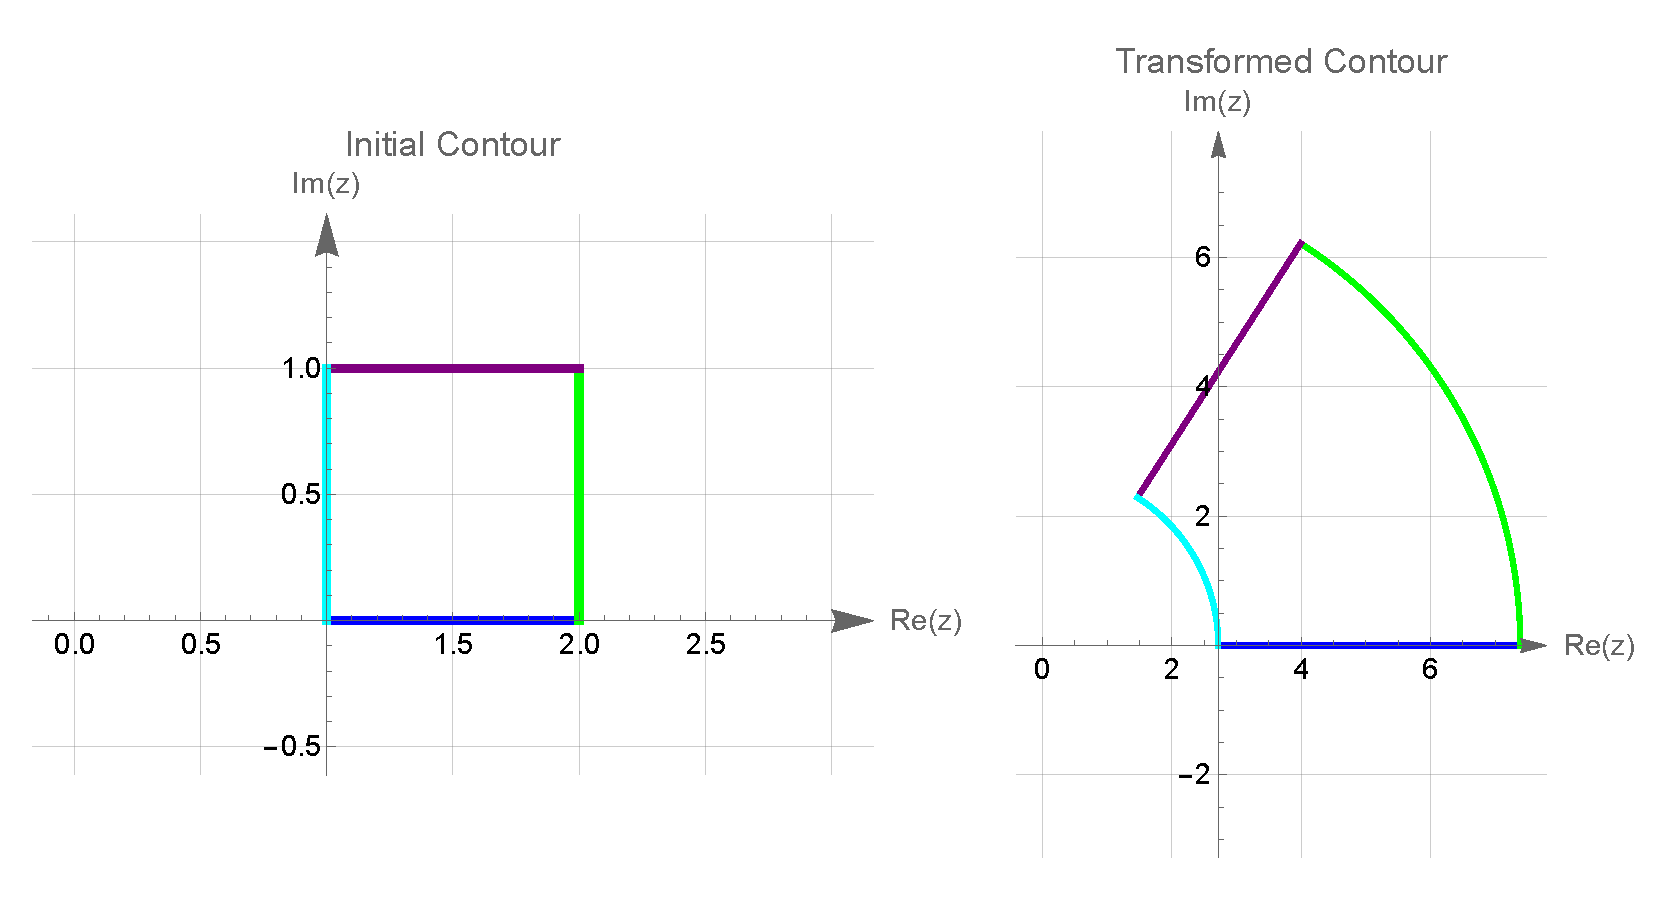
\includegraphics[width=\textwidth]{images/exam/transformation.pdf}
    \caption{Образ квадрата під дією відображення $\mathsf{Exp}: z \mapsto e^z$.}
    \label{fig:problem-4}
\end{figure}

\end{document}
